\chapter{Special Random Variables}


\begin{flushright}
	\textit{``Wow, this cumulative distribution function has a closed form expression!"} 
\end{flushright}

\textbf{Bernoulli RV} : Consider an experiment that only has two outcomes - success and failure. This can be represented by a RV that takes values $ \left\{0, 1\right\} $, with PMF

\begin{align}
	P \left\{X = 0\right\} &= 1-p \nonumber \\
	%
	P \left\{X = 1\right\} &= p \qquad \text{with} \qquad p \in [0, 1] \\
	%
	\mathbb{E}[X] &= p \\
	%
	\mathrm{Var}(X) &= p(1-p)
\end{align}

\textbf{Binomial RV} : Consider a set of $ n $ independent Bernoulli RVs. The total number of successes is called a Binomial RV, because of the PMF resembling binomial coefficients. This automatically makes the PMF defined only at non-negative integer values.

\begin{figure}[!h]
	\centering
	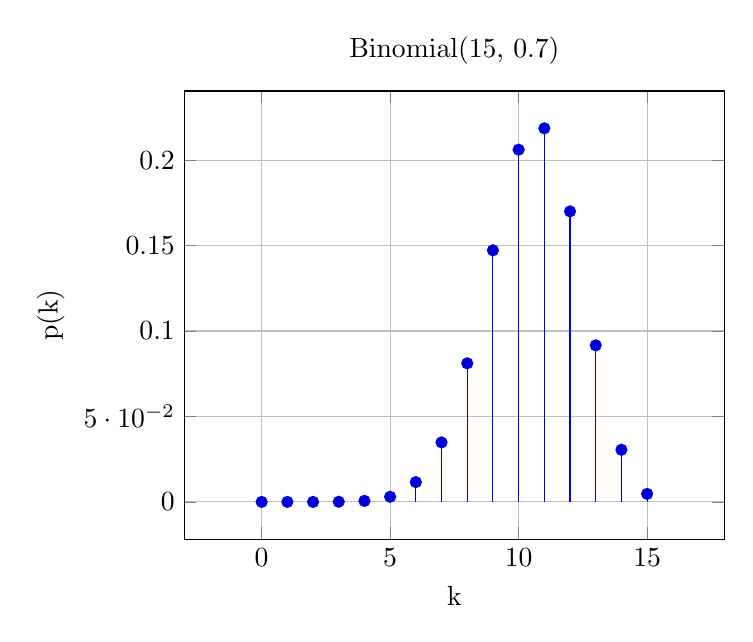
\begin{tikzpicture}
		\begin{axis}[enlarge x limits=0.2, grid = both,
			xlabel = k, ylabel = p(k), title = {Binomial(15, 0.7)}]
			\addplot+[ycomb] plot coordinates {( 0 , 0.0 ) ( 1 , 0.0 ) ( 2 , 0.0 ) ( 3 , 0.0001 ) ( 4 , 0.0006 ) ( 5 , 0.003 ) ( 6 , 0.0116 ) ( 7 , 0.0348 ) ( 8 , 0.0811 ) ( 9 , 0.1472 ) ( 10 , 0.2061 ) ( 11 , 0.2186 ) ( 12 , 0.17 ) ( 13 , 0.0916 ) ( 14 , 0.0305 ) ( 15 , 0.0047 ) };  
		\end{axis} 
	\end{tikzpicture}
\end{figure}


The two defining parameters of a Binomial RV are $ (n, p) $ where $ n $ is the number of trials and $ p $, the probability of each trial being independently a success.

\begin{align}
	P \left\{X = i\right\} &= \binom{n}{i}\ p^i \ (1-p)^{n-i}
\end{align}

Proving the normalization constraint requires the binomial theorem,
\begin{align}
	[p + (1-p)]^n &= 1^n = 1 \nonumber \\
	%
	\sum\limits_{i=0}^{n} P \left\{X = i\right\} &= \sum\limits_{i=0}^{n} \binom{n}{i}\ p^i \ (1-p)^{n-i}  = 1
\end{align}

Using the fact that the $ \mathbb{E}[\sum X] $ when the RVs are independent, reduces to $ \sum \mathbb{E}[X] $, and a similar rule for the variance,

\begin{align}
	\mathbb{E}[X] &= np \\
	%
	\mathrm{Var}(X) &= np(1-p)
\end{align}

If $ X_1, X_2 $ are two binomial RVs with parameters $ (n_1, p) $ and $ (n_2, p) $, then the RV $ X = X_1 + X_2 $ is also a binomial RV with parameters $ (n_1 + n_2, p) $ 

\textbf{Poisson RV} : Consider an RV that takes on non-negative integer values along with a parameter $ \lambda > 0 $, whose PMF is given by


\begin{align}
	P \left\{X = i\right\} &= e^{-\lambda}\ \frac{\lambda^i}{i!}
\end{align}

Using the Taylor series expansion of the exponential function, the normalization constraint is proved as follows,


\begin{align}
	e^x &= 0 + 1 + \frac{x^2}{2!} + \frac{x^3}{3!} + \dots \nonumber \\
	%
	\sum\limits_{i=0}^{\infty} P \left\{X = i\right\} &= e^{-\lambda} \left(\sum\limits_{i=0}^{\infty} \frac{\lambda^i}{i!}\right) = e^{-\lambda} \ e^{\lambda} = 1
\end{align}

\begin{figure}[!h]
	\centering
	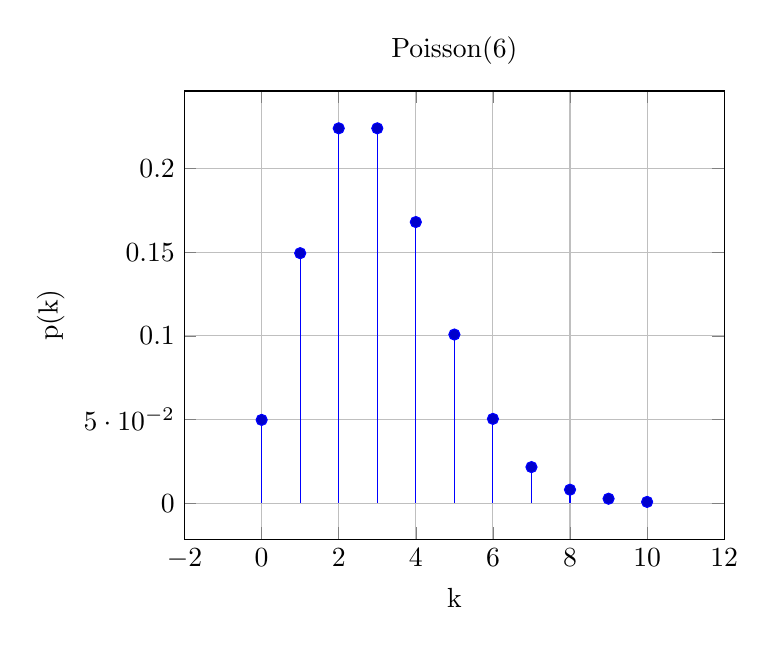
\begin{tikzpicture}
		\begin{axis}[enlarge x limits=0.2, grid = both,
			xlabel = k, ylabel = p(k), title = {Poisson(6)}]
			\addplot+[ycomb] plot coordinates {( 0 , 0.0498 ) ( 1 , 0.1494 ) ( 2 , 0.224 ) ( 3 , 0.224 ) ( 4 , 0.168 ) ( 5 , 0.1008 ) ( 6 , 0.0504 ) ( 7 , 0.0216 ) ( 8 , 0.0081 ) ( 9 , 0.0027 ) ( 10 , 0.0008 ) };  
		\end{axis} 
	\end{tikzpicture}
\end{figure}

Using the derivatives of the moment-generating function $ \phi(t) $, gives the mean and variance,

\begin{align}
	\phi(t) &= \mathbb{E}[e^{tX}] = \exp\left\{\lambda (e^t - 1)\right\}\\
	%
	\mathbb{E}[X] &= \lambda \\
	%
	\mathrm{Var}(X) &= \lambda
\end{align}

In the limit of $ n $ very large and $ p $ very small for a binomial RV with parameters $ (n, p) $, it can be approximated using a Poisson RV with parameter $ \lambda = np $.

\begin{align}
	P \left\{X = i\right\}\ =\ \binom{n}{i}\ p^i\ (1-p)^{n-i}\ \approxeq\ e^{-np}\ \frac{(np)^i}{i!}
\end{align}

An evern more general result, uses $ n $ independent trials each with probability of success $ p_i \ \forall\ i \in \left\{1, \dots, n\right\}$, with the condition that $ n $ is large and all of the $ p_i $ are small. The Poisson RV approximation can then me made with parameter $ \lambda = \sum p_i $.

Weak independence is measured by the conditional probability of one event succeeding given another has already succeeded. If these two values are approximately equal, then this approximation applies.

If $ X_1, X_2 $ are independently Poisson distributed with parameters $ \lambda_1, \lambda_2 $, then their sum $ X = X_1 + X_2 $ is also Poisson distributed with parameter $ \lambda_1 + \lambda_2 $. Since the moment generating function of a distribution uniquely determines it,

\begin{align}
	\phi (t) &= \mathbb{E}[e^{tX}] = \mathbb{E}[e^{t(X_1 + X_2)}] \nonumber \\
	%
	&= \mathbb{E}[e^{tX_1}] \mathbb{E}[e^{tX_2}] \nonumber \\
	%
	&= \exp\left\{(\lambda_1 + \lambda_2) (e^t - 1)\right\}
\end{align}

As an extension of the above, consider a total of $ N $ events, of which $ N_1, N_2 $ represent the number of events of types 1 and 2, with probabilities $ p $ and $ 1-p $ respectively. Also, $ N = N_1 + N_2 $.

If $ N $ is Poisson distributed with mean $\lambda$, then $ N_1, N_2 $ are also Poisson distributed with mean $ p\lambda $ and $ (1-p)\ \lambda $ respectively. This easily extends to more than two possible event types.

\begin{align}
	P\left\{N = n+m\right\} &= e^{-\lambda} \ \frac{\lambda^{n+m}}{(n+m)!} \nonumber \\
	%
	P\left\{N_1 = n\right\} &= e^{-p\lambda} \ \frac{(p\lambda)^{n}}{(n)!} \nonumber \\
	%
	P\left\{N_2 = m\right\} &= e^{-(1-p)\lambda} \ \frac{((1-p)\lambda)^{m}}{(m)!}
\end{align}

\textbf{Hypergeometric RV} : Consider a set of $ N+M $ objects of which $ N $ are acceptable and $ M $ defective. Let an experiment involve choosing $ n $ random objects out of $ N+M $, and then measure the number of acceptable objects picked using the RV $ X $.

$ X \in \left\{0, 1, \dots, \min(n, N) \right\} $, as the number of acceptable objects picked cannot exceed $ N $. This is a hypergeometric RV with PMF given by,

\begin{align}
	P \left\{X = i\right\} &= \ddfrac{\binom{N}{i}\ \binom{M}{n-i}}{\binom{N+M}{n}}
\end{align}

The parameters are $ (N, M, n) $, with the RV taking on non-negative integer values. If the proportion of acceptable objects is $ p $, then,

\begin{align}
	\mathbb{E}[X] &= \frac{nN}{N+M} = np \\
	%
	\mathrm{Var}(X) &= \frac{nNM}{(N+M)^2}\ \left(1 - \frac{n-1}{N+M-1}\right) \nonumber \\
	%
	&=  np\ (1-p)\ \left(1 - \frac{n-1}{N+M-1}\right)
\end{align}

Notice from the variance that the hypergeometric distribution converges to a binomial distribution in the limit $ N+M \to \infty $ and thus $ n \lll N $.

Consider two binomial RVs $ X, Y $ with parameters $ (n, p) $ and $ (m, p) $ respectively. The PMF of $ X $, given $ X+Y = k $ is given by,

\begin{align}
	P \left\{X = i\ |\ X+Y = k\right\} &= \ddfrac{\binom{n}{i}\ \binom{m}{k-i}}{\binom{n+m}{k}}
\end{align}

The denominator uses the fact that $ X+Y $ is also binomial with paramters $ (n+m, p) $, and the expression measures the probability that $ i $ out of the $ k $ successes were contributed by the RV $ X $.

This turns out to be a hypergeomtric RV measuring how many out of $ k $ objects picked were of type $ X $.


\textbf{Uniform RV} : Consider a continuous RV over the closed interval $ \left[\alpha, \beta\right] $, with PDF given by

\begin{align}
	f(x) &= \frac{1}{\beta - \alpha} & \text{if}\ x \in \left[\alpha, \beta\right] \\
	%
	f(x) &= 0 & \text{otherwise} \nonumber
\end{align}

The normalization constriant is easily proven using the Riemann integration of a continuous function.

\begin{align}
	P \left\{a < X < b\right\} &= \int\limits_{a}^{b} f(x)\ \mathrm{d} x = \frac{b - a}{\beta - \alpha} \\
	%
	P \left\{-\infty < X < \infty\right\} &= \int\limits_{-\infty}^{\infty} f(x)\ \mathrm{d} x = 1 \nonumber
\end{align}

Using simple polynomial integrations,

\begin{align}
	\mathbb{E}[X] &= \frac{\alpha + \beta}{2} \\
	%
	\mathrm{Var}(X) &= \frac{(\beta - \alpha)^2}{12} 
\end{align}


By computer science convention, a \textit{random number} is a uniformly distributed real number in the range $ [0, 1] $. A simple linear transformation $ Y = aX + b $ can be used to rescale this random number to the domain $ [b, a+b] $.

An important application of uniform RV sampling is Monte Carlo simulations, often used to estimate a parameter by performing a large number of experiments and using a frequentist approach to assign probabilities.

\textbf{Normal RV} : The most consistent distribution underlying real-world datasets, and as a result the most well-studied. This was originally introduced as an approximation to binomial distributions with extremely large $ n $. Using the mean and variance as parameters, the PDF for $ X \sim \mathcal{N}(\mu, \sigma^2) $ is defined as

\begin{align}
	f(x) = \frac{1}{\sqrt{2 \pi \sigma^2}} \exp \left[\frac{- (x - \mu)^2}{2\sigma^2}\right] \qquad \forall \quad x \in \mathbb{R}
\end{align}

This distribution is also called a bell curve. It is symmetric about $ \mu $, which is also its maximum.

\begin{align}
	\mathbb{E}[X] &= \mu \\
	%
	\mathrm{Var}(X) &= \sigma^2 \\
	%
	\mathbb{E}[aX + b] &= a\ \mu + b \nonumber \\
	%
	\mathrm{Var}(aX + b) &= a^2 \ \sigma^2 \nonumber 
\end{align}

\textit{Standard normal RV} : A normal RV with mean 0 and variance 1. Any normal RV $ X $ can be converted into a standard normal RV ($ \Phi $), using the transform $ Z = (X - \mu) / \sigma$

\begin{align}
	X &\sim \mathcal{N}(\mu, \sigma^2) \nonumber \\
	%
	Z &\sim \mathcal{N}(0, 1) \qquad \text{using} \qquad Z = \frac{X - \mu}{\sigma}
\end{align}

\begin{figure}[H]
	\centering
	\begin{tikzpicture}
		\begin{axis}[xlabel=$x$, grid = both, xmin = -3.5, xmax = 3.5, ylabel = {$f(x)$}, title = {$ Z \sim \mathcal{N}(0, 1) $}]
			\addplot[thick, smooth, draw=blue][name path = f2, domain = -4:4]{(1/sqrt(2*pi)*exp(-x*x*0.5))};
		\end{axis}
	\end{tikzpicture}
\end{figure}

The numerical value of the standard normal RV $ (\Phi) $ has historically been computed using approximations and the CDF tabulated to a high degree of precision. Such a reference table is used to actually assign probabilities to $ \Phi $ 

\begin{align}
	\Phi(x) &= \int\limits_{-\infty}^{x} \frac{1}{\sqrt{2 \pi}} \exp \left(\frac{-y^2}{2}\right)\ \mathrm{d}y \\
	%
	P\left\{X < b\right\} &= P \left\{\frac{X - \mu}{\sigma} < \frac{b - \mu}{\sigma}\right\} = \Phi \left\{\frac{b - \mu}{\sigma}\right\} \\
	%
	\Phi(-x) &= 1 - \Phi(x)
\end{align}

The moment generating function of a normal RV uses the result for a standard normal RV.

\begin{align}
	\phi_Z (t) &= \mathbb{E}[e^{tZ}] = \exp\left(\frac{t^2}{2}\right)	  \\
	%
	\phi_X (t) &= \mathbb{E}[e^{t\mu}\ e^{t \sigma Z}] = \exp\left(\mu t + \frac{\sigma^2 t^2}{2}\right)
\end{align}

This also leads to the fact that the sum of independent normal RVs is also a normal RV. Consider a set of normal RVs $ \left\{X_i\right\} $ with mean and variance $ \left\{\mu_i\right\},\ \left\{\sigma^2_i\right\} $ respectively. From the moment-generating function,

\begin{align}
	\mathbb{E}[e^{tX}] &= \prod_{i=1}^{n} \mathbb{E}[e^{tX_i}] \nonumber \\
	%
	\mu &= \sum\limits_{i=1}^{n} \mu_i \qquad \text{and} \qquad \sigma^2 = \sum\limits_{i=1}^{n} \sigma_i^2
\end{align}

\textit{Percentile and z-score} : By convention, $ \alpha $ and $ z_\alpha $ are called the \textit{p-value} and \textit{z-score} respectively. The $ 100 \alpha $ percentile of a standard normal RV is that value $ x = z_\alpha $ for which,

\begin{align}
	P \left\{Z > z_\alpha\right\} &= 1 - \Phi(z_\alpha) = \alpha
\end{align}

\begin{figure}[H]
	\centering
	\begin{tikzpicture}
		\begin{axis}[width = 0.75\textwidth,xlabel=$x$, ylabel=$ f(x) $, grid = both, xmin = -4.5, xmax = 4.5, title = {$z_\alpha = 1$, $ \alpha = 0.158 $}]
			\addplot[thick, smooth, draw=red][name path = f1, domain = -5:1]{(1/sqrt(2*pi)*exp(-x*x*0.5))};
			\addplot[thick, smooth, draw=blue][name path = f2, domain = 1:5]{(1/sqrt(2*pi)*exp(-x*x*0.5))};
			
			\path[name path=axis1] (axis cs:-5,0) -- (axis cs:1,0);
			\path[name path=axis2] (axis cs:1,0) -- (axis cs:5,0);
			
			\addplot [thick,color=red,fill=red, fill opacity=0.1] fill between[of=f1 and axis1,];
			\addplot [thick,color=red,fill=blue, fill opacity=0.1] fill between[of=f2 and axis2,];
			
			\node[color=blue, fill=white] at (axis cs: 1.5,.05) {$ \alpha $};
			\node[color=red, fill=white] at (axis cs: -0.5,.05) {$ 1 - \alpha $};
			
		\end{axis}
	\end{tikzpicture}
\end{figure}


\textbf{Exponential RV} :  Consider a continuous RV defined over the real line with PDF and CDF given by

\begin{align}
	f(x) &= \lambda\ e^{-\lambda x} & \text{if}\ x \in \left[0, \infty\right) \\
	%
	f(x) &= 0 & \text{otherwise} \nonumber
\end{align}


\begin{figure}[H]
	\begin{tikzpicture}
		\begin{axis}[xlabel=$x$, grid = both, xmin = -1.5, xmax = 4.5, title = {$f(x)$}]
			\addplot[thick, smooth, draw=blue][name path = f1, domain = -2:0]{0};
			\addplot[thick, smooth, draw=blue][name path = f1, domain = 0:5]{2*exp(-2*x)};
			\addlegendentry{$ \lambda = 2$}
		\end{axis}
	\end{tikzpicture}
	%
	\begin{tikzpicture}
		\begin{axis}[xlabel=$x$, grid = both, xmin = -1.5, xmax = 4.5, title = {$F(x)$}, legend pos = north west]
			\addplot[thick, smooth, draw=red][name path = f1, domain = -2:0]{0};
			\addplot[thick, smooth, draw=red][name path = f1, domain = 0:5]{1 - exp(-2*x)};
			\addlegendentry{$ \lambda = 2$}
		\end{axis}
	\end{tikzpicture}
\end{figure}


The parameter $ \lambda $ , called the \textit{rate}, solely defines the exponential RV with a CDF,

\begin{align}
	F(x) &= 1 - e^{-\lambda x} \qquad \forall \ x \geq 0
\end{align}

The exponential distribution if observed most commonly as the distribution of time intervals between successive occurrences of natural events. The moment-generating function gives the mean and variance as follows

\begin{align}
	\phi(t) &= \frac{\lambda}{\lambda - t} \qquad \forall\ t < \lambda \\
	%
	\mathbb{E}[X] &= \frac{1}{\lambda} \\
	%
	\mathrm{Var}(X) &= \frac{1}{\lambda^2}
\end{align}

An important property exclusive to the exponential function is that it is \textit{memoryless}, or \textit{self-similar} across time. This is mathematically represented as

\begin{align}
	P \left\{X > t+s\ |\ X > t \right\} &= P \left\{X > s \right\} \qquad \forall \ s, t\geq 0
\end{align}

The probability of an item functioning for $ s $ additional time does not depend on the fact that it has functioned for $ t $ time already.

The minimum of a set of independent exponential RVs $ \left\{X_i\right\} $ with parameters $ \left\{\lambda_i\right\} $ is also an exponential RV. This is easily understood as the lifetime of a system with many components all of which are necessary for it to function.

\begin{align}
	P \left\{\mathrm{min}(X_1, X_2, \dots, X_n) > x\right\} &= e^{-\lambda x} \nonumber \\
	%
	\lambda &= \sum_{i=1}^{n} \lambda_i
\end{align}

An independent exponential RV transforming as $ X \to cX $ causes the rate to change as $ \lambda \to \lambda/c $.

\textbf{Poisson process} : Consider a process where events happen randomly such that $ N(t) $ denotes the number of events in the time $ [0, t] $. This is a Poisson process with \textit{rate} $ \lambda $, if

\begin{itemize}
	\item $ N(0) = 0 $, with $ t = 0 $ denoting the start of the process.
	
	\item Disjoint time intervals have an independent number of events occurring in them.
	
	\item The number of events in a given interval has a distribution depending only on the length of the interval.
	
	\item In the limit of a small time interval of length $ h \to 0 $, the probability of event occurrence
	
	\begin{align}
		P \left\{N(h) = 1\right\} &\approx \lambda h \nonumber \\
		%
		P \left\{N(h) \geq 2\right\} &\approx 0
	\end{align}
\end{itemize}

The distribution of the number of events occurring in any interval of length $ t $ in a Poisson process is a Poisson RV with parameter $ \lambda t $.

\begin{align}
	P \left\{N(t) = k\right\} &= e^{-\lambda t} \ \frac{(\lambda t)^k}{k!}
\end{align}

For a Poisson process, let $ Y_n $ denote the time interval between the $ (n-1)^{th} $ and $ n^{th} $ events for all $ n > 1 $. This set $ \left\{Y_n\right\} $ is called \textit{inter-arrival time}. Then, the set $ Y_n $ are all independent RVs having an exponential distribution with parameter $ \lambda $ 

\textbf{Pareto RV} : Using the self-similarity of the exponential RV, the Pareto distribution is used to exmaine the distribution of income among a population and to identify what proportion of the total income earned by a population is contributed by the top earners.

Consider an exponential RV $ X $ with rate $ \lambda $. The Pareto RV with minimum parameter $ \alpha $ and index parameter $ \lambda > 0$, is given by

\begin{align}
	Y &= \alpha\ e^{X} \\
	%
	X &= \lambda\ e^{-\lambda x} & \text{if}\ x \in \left[0, \infty\right) \nonumber
\end{align}

This RV is constrained by $ Y \geq \alpha $. The CDF of the Pareto distribution is

\begin{align}
	P \left\{Y > y\right\} &= \left(\frac{\alpha}{y}\right)^\lambda \nonumber \\
	%
	F_Y(y) &= 1 - \left(\frac{\alpha}{y}\right)^\lambda \qquad \forall \  y \geq \alpha \\
	%
	f_Y(y) &= \frac{\lambda}{y}\ \left(\frac{\alpha}{y}\right)^\lambda \qquad \forall \  y \geq \alpha
\end{align}

\begin{figure}[H]
	\begin{tikzpicture}
		\begin{axis}[xlabel=$x$, grid = both, xmin = 1.5, xmax = 5.5, title = {$f(x)$}]
			\addplot[thick, smooth, draw=blue][name path = f1, domain = 0:2]{0};
			\addplot[thick, smooth, draw=blue][name path = f1, domain = 2:6]{8/(x^(3))};
			\addlegendentry{$ \alpha, \lambda = 2$}
		\end{axis}
	\end{tikzpicture}
	%
	\begin{tikzpicture}
		\begin{axis}[xlabel=$x$, grid = both, xmin = 1.5, xmax = 5.5, title = {$F(x)$}, legend pos = north west]
			\addplot[thick, smooth, draw=red][name path = f1, domain = 0:2]{0};
			\addplot[thick, smooth, draw=red][name path = f1, domain = 2:6]{1 - (2/x)^2};
			\addlegendentry{$ \alpha, \lambda = 2$}
		\end{axis}
	\end{tikzpicture}
\end{figure}

The expected value is finite only for $ \lambda > 1 $,

\begin{align}
	\mathbb{E}(Y) &= \alpha \ \frac{\lambda}{\lambda - 1 }
\end{align}

As a result of the self-similarity of the exponential distribution, the Pareto RV is also self-similar. Given the condition $ Y > y_0 $ for some $ y_0 > \alpha $, this conditional distribution is also Pareto with parameters $ y_0 $ and $ \lambda $.

\begin{align}
	P \left\{Y > y\ |\ Y > y_0 \right\} = \left(\frac{y_0}{y}\right)^\lambda
\end{align}

\textbf{Gamma distribution} : Consider the gamma function $ \Gamma(x) $ defined by an integral which can be recursively related to itself.

\begin{align}
	\Gamma(\alpha) &= \int\limits_{0}^{\infty} e^{-y}\ y^{\alpha -1}\ \mathrm{d}y \\
	%
	\Gamma(\alpha) &= (\alpha - 1)\ \Gamma(\alpha - 1)
\end{align}

For the special case of integer values of $ \alpha $, and using $ \Gamma(1) = 1 $,
\begin{align}
	\Gamma(n) &= (n - 1)\ \Gamma(n - 1) \nonumber \\
	%
	\Gamma(n) &= (n-1)!	
\end{align}

The Gamma RV with parameters $ \alpha, \lambda > 0 $, is now defined using the PDF,

\begin{align}
	f(x) &= \lambda\ e^{- \lambda x}\ \frac{(\lambda x)^{\alpha-1}}{\Gamma(\alpha)} \qquad \forall\ x \geq 0 \\
	%
	&= 0 \qquad \text{otherwise} \nonumber
\end{align}

\begin{figure}[H]
	\centering
	\begin{tikzpicture}
		\begin{axis}[width = 0.75\textwidth,xlabel=$x$, ylabel=$ f(x) $, grid = both, xmin = -0.5, xmax = 20]
			\addplot[thick, smooth, draw=black][name path = f1, domain = -1:0]{0};
			\addplot[thick, smooth, draw=blue][name path = f2, domain = 0:20]{e^(-x)*x};
			\addplot[thick, smooth, draw=green][name path = f3, domain = 0:20]{e^(-x)*(x^3)/6};
			\addplot[thick, smooth, draw=orange][name path = f4, domain = 0:20]{e^(-x)*(x^7)/5040};
			\addplot[thick, smooth, draw=red][name path = f5, domain = 0:20]{e^(-x)*(x^15)/1307674368000};
			\legend{$ \alpha = 2 $, $ \alpha = 4 $, $ \alpha = 8 $, $ \alpha = 16 $}
		\end{axis}
	\end{tikzpicture}
\end{figure}



The moment-generating function gives the mean and variance using

\begin{align}
	\phi(t) &= \left(\frac{\lambda}{\lambda - t}\right)^{\alpha} \\
	%
	\mathbb{E}[X] &= \frac{\alpha}{\lambda} \\
	%
	\mathrm{Var}(X) &= \frac{\alpha}{\lambda^2}
\end{align}

Using the moment-generating function above, the sum of many independent Gamma RVs $ \left\{X_i\right\} $ with parameters $ \left\{\alpha_i\right\} $ and a shared $ \lambda $, then their sum $ X = \sum X_i $ is also a Gamma RV with parameters $ \sum \alpha_i $ and $\lambda$.

This result further simplifies when $ \alpha = 1 $, making the Gamma RVs reduce to exponential RVs with the same rate parameter $ \lambda $. The sum of $ n $ independent exponential RVs $ \left\{X_i\right\} $ with a shared rate $ \lambda $, is a Gamma RV with parameters $ (n, \lambda) $.

Note the effect of multiplying a Gamma RV by a scalar. Let $ X $ be a Gamma RV which is multiplied by scalar $ b $, Now the moment-generating function of the new RV $ bX $ is

\begin{align}
	\mathbb{E}[e^{tX}] &= \left(\frac{\lambda}{\lambda - t}\right)^\alpha \nonumber \\
	%
	\mathbb{E}[e^{t\ bX}] &= \mathbb{E}[e^{bt\ X}] = \left(\frac{\lambda}{\lambda - bt}\right)^\alpha = \left(\frac{\lambda / b}{\lambda / b - t}\right)^\alpha \nonumber \\
	%
	bX &\sim \Gamma(\alpha, \lambda / b)  \qquad \text{if} \qquad X \sim \Gamma(\alpha, \lambda)
\end{align}

\textbf{Chi-square distribution} : Consider a set of independent standard normal RVs $ \left\{Z_i\right\} $. Then the RV defined as $ X \sim \chi_n^2 $ is given by

\begin{align}
	X = Z_1^2 + Z_2^2 + \dots + Z_n^2
\end{align}

$ X $ is a chi-squared RV with $ n $ \textit{degrees of freedom}. Similar to the p-value from the normal RV, $ \chi_{\alpha, n}^2 $ is defined as follows and tabulated using approximate computations.

\begin{align}
	P \left\{X \geq \chi_{\alpha, n}^2 \right\} = \alpha
\end{align}

The equivalence of the chi-squared and Gamma distributions can be seen through the moment-generating functions 

\begin{align}
	\phi(t) &= (1-2t)^{-n/2} \\
	%
	\phi(t) &= \left(\frac{1/2}{1/2 - t}\right)^{n/2} \nonumber
\end{align}

Thus, a chi-squared RV with $ n $ degrees of freedom is the same as a Gamma distribution with parameters $ (n/2, 1/2) $.

\begin{align}
	\mathbb{E}[X] &= \frac{n/2}{1/2} = n \\
	%
	\mathrm{Var}(X) &= \frac{n/2}{(1/2)^2} = 2n
\end{align}

\textbf{t-distribution} : Using a standard normal RV $ Z $ and a chi-square RV $ \chi_n^2 $ with $ n $ degrees of freedom, the t-distribution is defined as,

\begin{align}
	T_n = \frac{Z}{\sqrt{\chi_n^2 / n}}
\end{align}

The t-distribution is also symmetric about $ x=0 $ like $ Z $, but with longer tails. It increasingly resembles $ Z $ as $ n \to \infty $. To prove this, use the weak law of large numbers on the denominator above.

\begin{align}
	\mathbb{E}[X] &= 0 \qquad n>1 \\
	%
	\mathrm{Var}(X) &= \frac{n}{n-2} \qquad n>2
\end{align}

Similar to the p-value from the normal RV, $ t_{\alpha, n} $ is defined as follows and tabulated using approximate computations.

\begin{align}
	P \left\{T_n \geq t_{\alpha, n} \right\} &= \alpha \\
	%
	t_{1-\alpha, n} &= -t_{\alpha, n} \nonumber
\end{align}

\textbf{F-distribution} : Let $ \chi_n^2, \chi_m^2 $ be chi-square RVs with $ n, m $ degrees of freedom respectively. Then,

\begin{align}
	F_{n,m} = \frac{\chi_n^2 / n}{\chi_m^2 / m}
\end{align}

is an F-distribution with$ n,m $ degrees of freedom.

Similar to the p-value from the normal RV, $ F_{\alpha, n, m} $ is defined as follows and tabulated using approximate computations.

\begin{align}
	P \left\{F_{n,m} \geq F_{\alpha, n, m} \right\} &= \alpha \\
\end{align}

\newpage

